%%%%%%%%%%%%%%%%%%%%%%%%%%%%%%%%%%%%%%%%%
% "ModernCV" CV and Cover Letter
% LaTeX Template
% Version 1.2 (25/3/16)
%
% This template has been downloaded from:
% http://www.LaTeXTemplates.com
%
% Original author:
% Xavier Danaux (xdanaux@gmail.com) with modifications by:
% Vel (vel@latextemplates.com)
%
% License:
% CC BY-NC-SA 3.0 (http://creativecommons.org/licenses/by-nc-sa/3.0/)
%
% Important note:
% This template requires the moderncv.cls and .sty files to be in the same 
% directory as this .tex file. These files provide the resume style and themes 
% used for structuring the document.
%
%%%%%%%%%%%%%%%%%%%%%%%%%%%%%%%%%%%%%%%%%

%----------------------------------------------------------------------------------------
%	PACKAGES AND OTHER DOCUMENT CONFIGURATIONS
%----------------------------------------------------------------------------------------

\documentclass[11pt,a4paper,sans]{moderncv} % Font sizes: 10, 11, or 12; paper sizes: a4paper, letterpaper, a5paper, legalpaper, executivepaper or landscape; font families: sans or roman
\usepackage[utf8]{inputenc}

\moderncvstyle{casual} % CV theme - options include: 'casual' (default), 'classic', 'oldstyle' and 'banking'
\moderncvcolor{blue} % CV color - options include: 'blue' (default), 'orange', 'green', 'red', 'purple', 'grey' and 'black'

\usepackage{lipsum} % Used for inserting dummy 'Lorem ipsum' text into the template

\usepackage[scale=0.75]{geometry} % Reduce document margins
%\setlength{\hintscolumnwidth}{3cm} % Uncomment to change the width of the dates column
%\setlength{\makecvtitlenamewidth}{10cm} % For the 'classic' style, uncomment to adjust the width of the space allocated to your name

%----------------------------------------------------------------------------------------
%	NAME AND CONTACT INFORMATION SECTION
%----------------------------------------------------------------------------------------

\firstname{Imanol} % Your first name
\familyname{Studer} % Your last name

% All information in this block is optional, comment out any lines you don't need
\title{Curriculum Vitae}
\address{Wickenweg 51}{8048 Zürich}
\mobile{+41 (0)76 462 67 16}
% \phone{}
% \fax{}
\email{imanol.studer@gmail.com}
% \homepage{}{} % The first argument is the url for the clickable link, the second argument is the url displayed in the template - this allows special characters to be displayed such as the tilde in this example
% \extrainfo{}
\photo[70pt][0.4pt]{pictures/picture} % The first bracket is the picture height, the second is the thickness of the frame around the picture (0pt for no frame)
% \quote{}

%----------------------------------------------------------------------------------------

\begin{document}

%----------------------------------------------------------------------------------------
%	COVER LETTER
%----------------------------------------------------------------------------------------

% To remove the cover letter, comment out this entire block

\clearpage

\recipient{HR Department}{Corporation\\123 Pleasant Lane\\12345 City, State} % Letter recipient
\date{\today} % Letter date
\opening{Sehr geehrte Damen und Herren,} % Opening greeting
\closing{Mit freundlichen Grüssen,} % Closing phrase
\enclosure[Anhang]{Lebenslauf, Master Noten, Bachelor Diplom} % List of enclosed documents

\makelettertitle % Print letter title

\lipsum[1-3] % Dummy text

\makeletterclosing % Print letter signature

%%%%%%%%%%%%%%%%%%%%%%%%%%%%%%%%%%%%%%%%%
% "ModernCV" CV and Cover Letter
% LaTeX Template
% Version 1.2 (25/3/16)
%
% This template has been downloaded from:
% http://www.LaTeXTemplates.com
%
% Original author:
% Xavier Danaux (xdanaux@gmail.com) with modifications by:
% Vel (vel@latextemplates.com)
%
% License:
% CC BY-NC-SA 3.0 (http://creativecommons.org/licenses/by-nc-sa/3.0/)
%
% Important note:
% This template requires the moderncv.cls and .sty files to be in the same 
% directory as this .tex file. These files provide the resume style and themes 
% used for structuring the document.
%
%%%%%%%%%%%%%%%%%%%%%%%%%%%%%%%%%%%%%%%%%

%----------------------------------------------------------------------------------------
%	PACKAGES AND OTHER DOCUMENT CONFIGURATIONS
%----------------------------------------------------------------------------------------

\documentclass[11pt,a4paper,sans]{moderncv} % Font sizes: 10, 11, or 12; paper sizes: a4paper, letterpaper, a5paper, legalpaper, executivepaper or landscape; font families: sans or roman
\usepackage[utf8]{inputenc}

\moderncvstyle{casual} % CV theme - options include: 'casual' (default), 'classic', 'oldstyle' and 'banking'
\moderncvcolor{blue} % CV color - options include: 'blue' (default), 'orange', 'green', 'red', 'purple', 'grey' and 'black'

\usepackage{lipsum} % Used for inserting dummy 'Lorem ipsum' text into the template

\usepackage[scale=0.75]{geometry} % Reduce document margins
%\setlength{\hintscolumnwidth}{3cm} % Uncomment to change the width of the dates column
%\setlength{\makecvtitlenamewidth}{10cm} % For the 'classic' style, uncomment to adjust the width of the space allocated to your name

%----------------------------------------------------------------------------------------
%	NAME AND CONTACT INFORMATION SECTION
%----------------------------------------------------------------------------------------

\firstname{Imanol} % Your first name
\familyname{Studer} % Your last name

% All information in this block is optional, comment out any lines you don't need
\title{Curriculum Vitae}
\address{Wickenweg 51}{8048 Zürich}
\mobile{+41 (0)76 462 67 16}
% \phone{}
% \fax{}
\email{imanol.studer@gmail.com}
% \homepage{}{} % The first argument is the url for the clickable link, the second argument is the url displayed in the template - this allows special characters to be displayed such as the tilde in this example
% \extrainfo{}
\photo[70pt][0.4pt]{pictures/picture} % The first bracket is the picture height, the second is the thickness of the frame around the picture (0pt for no frame)
% \quote{}

%----------------------------------------------------------------------------------------

\begin{document}

%----------------------------------------------------------------------------------------
%	COVER LETTER
%----------------------------------------------------------------------------------------

% To remove the cover letter, comment out this entire block

%\clearpage
%
%\recipient{HR Department}{Corporation\\123 Pleasant Lane\\12345 City, State} % Letter recipient
%\date{\today} % Letter date
%\opening{Dear Sir or Madam,} % Opening greeting
%\closing{Sincerely yours,} % Closing phrase
%\enclosure[Attached]{curriculum vit\ae{}, Master Grades, Bachelor's Diploma} % List of enclosed documents
%
%\makelettertitle % Print letter title
%
%\lipsum[1-3] % Dummy text
%
%\makeletterclosing % Print letter signature
%
%\newpage
%----------------------------------------------------------------------------------------
%	CURRICULUM VITAE
%----------------------------------------------------------------------------------------

\makecvtitle % Print the CV title

%----------------------------------------------------------------------------------------
%	EDUCATION SECTION
%----------------------------------------------------------------------------------------

\section{Ausbildung}

\cventry{2014--2016}{Master of Science - Multimodal and Cognitive Systems}{Universität Zürich}{}{}{Beinhaltet folgende Module:
\begin{itemize}
	\item Fundamentals of Image Processing and Computer Vision
	\item Autonomous Mobile Robots
	\item Introduction to Machine Learning (ETH Course)
	\item Neuromorphic Engineering II
	\item Neurophysics
	\item Complex Systems: Berechenbares Chaos in dynamischen Systemen
	\item Master Project: Head Pose Tracking with Quadrotors with Headmounted camera
\end{itemize}}  % Arguments not required can be left empty

\cventry{2009--2013}{Bachelor of Science - Angewandte Informatik: Neuroinformatics}{Universität Zürich}{}{}{Beinhaltet folgende Module:
\begin{itemize}
	\item Neuromorphic Engineering I
	\item Theory, Programming and Simulation of Neural Networks
	\item Systems Neuroscience
	\item Computational Vision
	\item Introduction to Neuroinformatics
\end{itemize}}

\cventry{2008--2009}{Passerelle}{AKAD College}{}{}{Die Passerelle ist eine Prüfung, welche dem Besitzer, zusammen mit einer Berufsmatura, zur Hochschulreife verhilft.}

\cventry{2003--2007}{Informatikmittelschule}{Kantonsschule Enge}{}{}{
Die Informatikmittelschule ist eine Ausbildung als Applikationsentwickler, ähnlich einer Lehre. Die Ausbildung besteht aus drei Jahren Schule, welche die üblichen Schulfächer abdeckt mit einem Fokus auf Betriebsökonomie. Das vierte und letzte Jahr ist ein Praktikum, währenddessen man eine zweiwöchige IPA (Individuelle Praktische Arbeit) absolvieren muss. Mein Projekt war ein Prototyp eines chemischen Monitoring Systems für Kläranlagen.}

\cventry{1999--2003}{Gymnasium, Altsprachliches Profil}{Kantonsschule Freudenberg}{}{}{Ich habe 4 Jahre Gymnasium mit einem Fokus auf Sprachen (Deutsch, Französisch, Spanisch, Latein) absolviert und dann zu Gunsten einer Ausbildung an der Informatikmittelschule abgebrochen.}

\section{Master Arbeit}

\cvitem{Title}{\emph{Paper Tracking} - A real time algorithm}
\cvitem{Supervisor}{Prof. Dr. Chat Wacharamanotham}
\cvitem{Description}{Ich habe einen Algorithmus entwickelt, welcher dazu in der Lage ist ein Paper in einem Bild zu finden, das von einer Kamera aufgenommen wurde, welche auf der Stirn des Lesers Montiert ist. Der Algorithmus sucht nach Bereichen in denen eine hohe Dichte von hohen Frequenzen gefunden werden. Das so gefundene Paper wird dann gegen eine PDF Datenbank gematcht mit Hilfe von SURF Features. Zuletzt wird dann die gematchte PDF Seite nach statistischen Grafiken abgesucht unter verwendung von Visual Words basierten Feature Vektoren und einer SVM mit einem RBF Kernel.}
\cvitem{Grade}{\textbf{5.75}}

\section{Bachelor Arbeit}

\cvitem{Title}{\emph{Maggie} - An Infant Robot Model}
\cvitem{Supervisor}{Dr. Hugo Gravato Marques}
\cvitem{Description}{I built a physical prototype of an infant robot model including an API to control it from a PC and collect data. It is made out of spare metal parts, servo motors, force resisting sensors, two cameras, IMUs and 3D designed and printed parts.}
\cvitem{Grade}{\textbf{5.5}}

%----------------------------------------------------------------------------------------
%	WORK EXPERIENCE SECTION
%----------------------------------------------------------------------------------------

\section{Arbeitserfahrung}

\cventry{2016--now}{Software Entwickler}{\textsc{Supercomputing Systems AG}}{Zürich}{}{Supercomputing Systems AG which developes outsourced software projects. During my time there I have been involved in the following projects as a software developer:
\begin{itemize}
	\item Gridsense: We developed a control software for electrical home devices that optimizes the power consumption of a household to minimize voltage variation in the power grid. I was responsible for the Software Architecture and IoT interface of the controllers.
	\item Smartbox: The smartbox is a smart sensor that is placed on transformer stations and can be used to optimize the balance of power load in the electrical grid of a region. I was responsible for the development of different modules.
	\item Renesas DNN: A Python interface to a neural network accelerator that is used in onboard car computers by different german car manufacturers. We implemented a software which converts trained networks to a architecture that fits the accelerator's specification. We also added floating-to-fixpoint conversion. My responsibility was to split the neural network convolutions into smaller operations and the fixpoint optimization part.
	\item Rega Cell phone detector: We developed a simple case-study-prototype for rega which determines the direction of a cellphone using two antennas. I was responsible for the part that localizes the direction and plots the results on a map.
	\item Transformation Tool for Schematics: Supercomputing Systems is developing a new railway controller based on FPGAs to replace the old ones. For this purpose we need an Editor that can be used to draw electrical schematics and convert them to VHDL code. I was responsible for programming the GUI using JavaFX.
\end{itemize}
}

\cventry{2012--2015}{Software Entwickler}{\textsc{New Voice AG}}{Zürich}{}{New Voice AG is a company located in Zürich which develops a software called MobiCall which is an Alarm-, Information-, Conference and Callrecording system which is built on top of a PBX system. My responsibility was to develop and maintain a plugin for locating Dect and WiFi devices inside buildings and triggering alarms.}

%------------------------------------------------

\cventry{2011--2012}{Software Entwickler}{\textsc{TrueBPM Solutions AG}}{Zürich}{}{TrueBPM develops a BPM system that is used internally by an assurance company. While I was working there, I was responsible for letter generation. I had to design BIRT reports based on word documents and also do some server backend programming. I left the company after a year, because the project was finished and I wanted to do something more challenging.}

%------------------------------------------------

\cventry{2006--2011}{Software Entwickler}{\textsc{IT-GR GmbH}}{Zürich}{}{IT-Gr GmbH is a software developing company. During my time there I worked alone on a monitoring system for water recycling plants for a customer called Unimon GmbH. The software periodically pulls measured data from different sensors embedded in the water plant. Users can log in through a web interface, analyze the data and create reports. It is also possible to define conditions under which alarms are  triggered. It then automatically contacts the responsible person per E-Mail or SMS.
\newline
My first year there (2006-2007) was an Internship as part of the “Informatikmittelschule”.}

%----------------------------------------------------------------------------------------

%----------------------------------------------------------------------------------------
%	REFERENCE CONTACTS SECTION
%----------------------------------------------------------------------------------------

\newpage

\section{Referenzpersonen}

\subsection{Prof. Dr. Chat Wacharamanotham}
\cvitem{Link}{\href{http://www.ifi.uzh.ch/en/zpac/people/chat.html}{http://www.ifi.uzh.ch/en/zpac/people/chat.html}}
\cvitem{}{Supervision of Master Thesis}
\cvitem{E-Mail}{\href{mailto:chat@ifi.uzh.ch}{chat@ifi.uzh.ch}}
\cvitem{Telephon}{+41 (0)44 635 43 13}

%----------------------------------------------------------------------------------------
%	COMPUTER SKILLS SECTION
%----------------------------------------------------------------------------------------

\section{Computer skills}

\cvitem{Basic}{\textsc{Bash Scripts}, QT, Cuda}
\cvitem{Intermediate}{\textsc{java}, \textsc{html}, \textsc{JavaScript}, \LaTeX, Microsoft Windows, OpenCV, Computer Hardware, Scikit Learn}
\cvitem{Advanced}{\textsc{python}, \textsc{C++}, Linux}

%----------------------------------------------------------------------------------------
%	LANGUAGES SECTION
%----------------------------------------------------------------------------------------

\section{Sprachen}

\cvitemwithcomment{Deutsch}{Muttersprache}{}
\cvitemwithcomment{Spanisch}{Muttersprache}{}
\cvitemwithcomment{Englisch}{Gut}{}
\cvitemwithcomment{Französisch}{Grundlagen}{}

%----------------------------------------------------------------------------------------

%----------------------------------------------------------------------------------------
%	INTERESTS SECTION
%----------------------------------------------------------------------------------------

\section{Interessen}

\renewcommand{\listitemsymbol}{-~} % Changes the symbol used for lists

\cvlistdoubleitem{Reading}{Jiu Jitsu}
\cvlistdoubleitem{Karate}{Cooking}
\cvlistdoubleitem{Workout}{Swimming}

\newgeometry{bottom=0pt}
\section{Master Diplom}
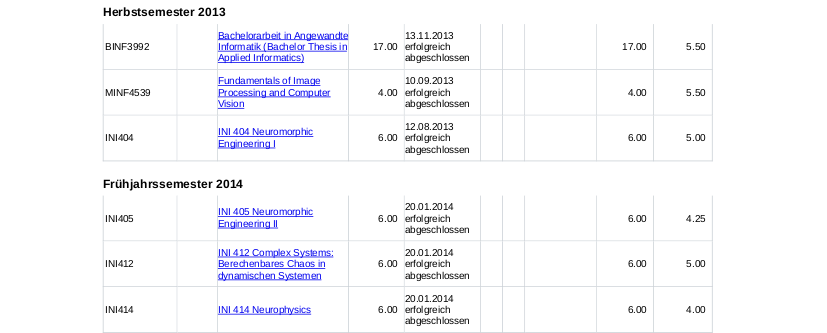
\includegraphics[width=\textwidth]{pictures/master/module1.png}
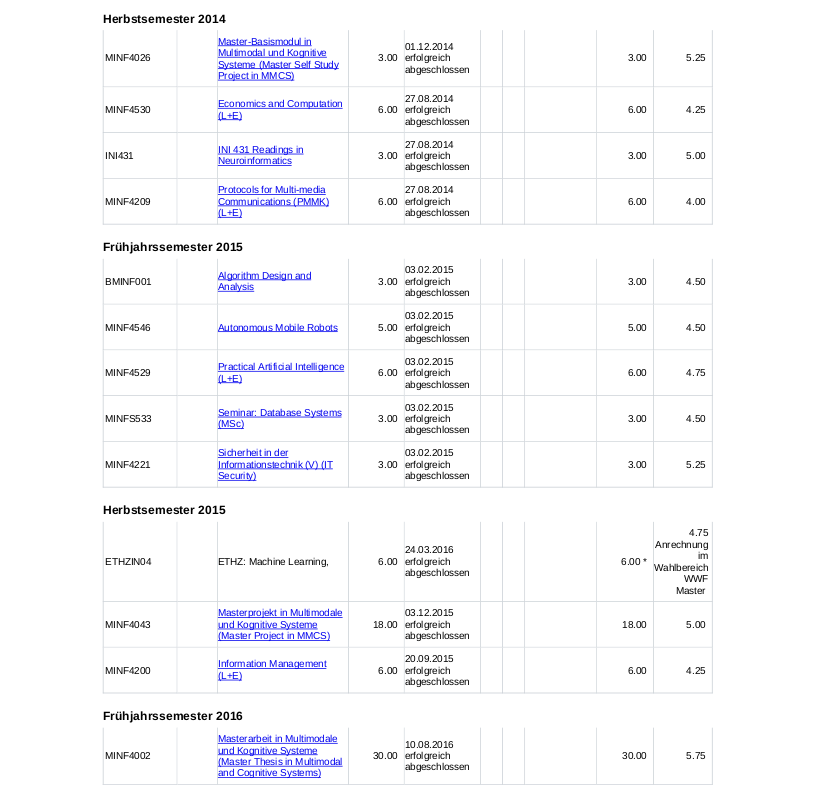
\includegraphics[width=\textwidth]{pictures/master/module2.png}

\enlargethispage{12pt}
\newpage
\section{Bachelor Diplom}
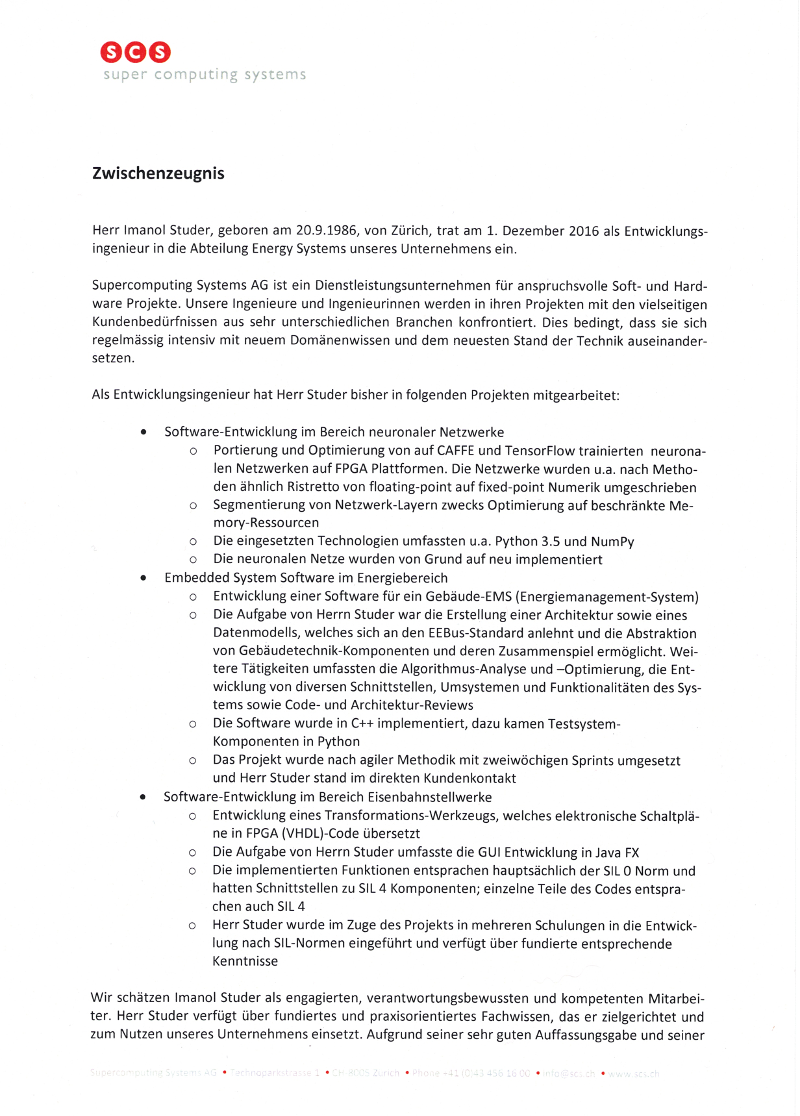
\includegraphics[width=\textwidth]{pictures/bachelor/page0.png}
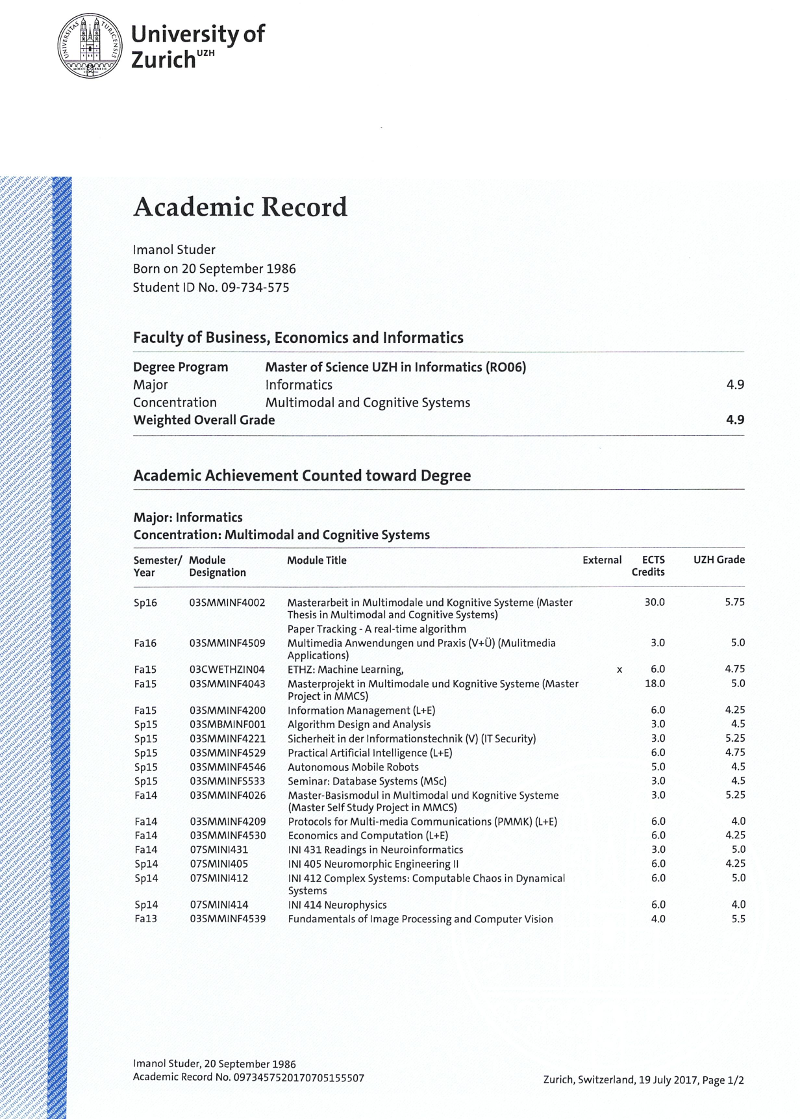
\includegraphics[width=\textwidth]{pictures/bachelor/page1.png}
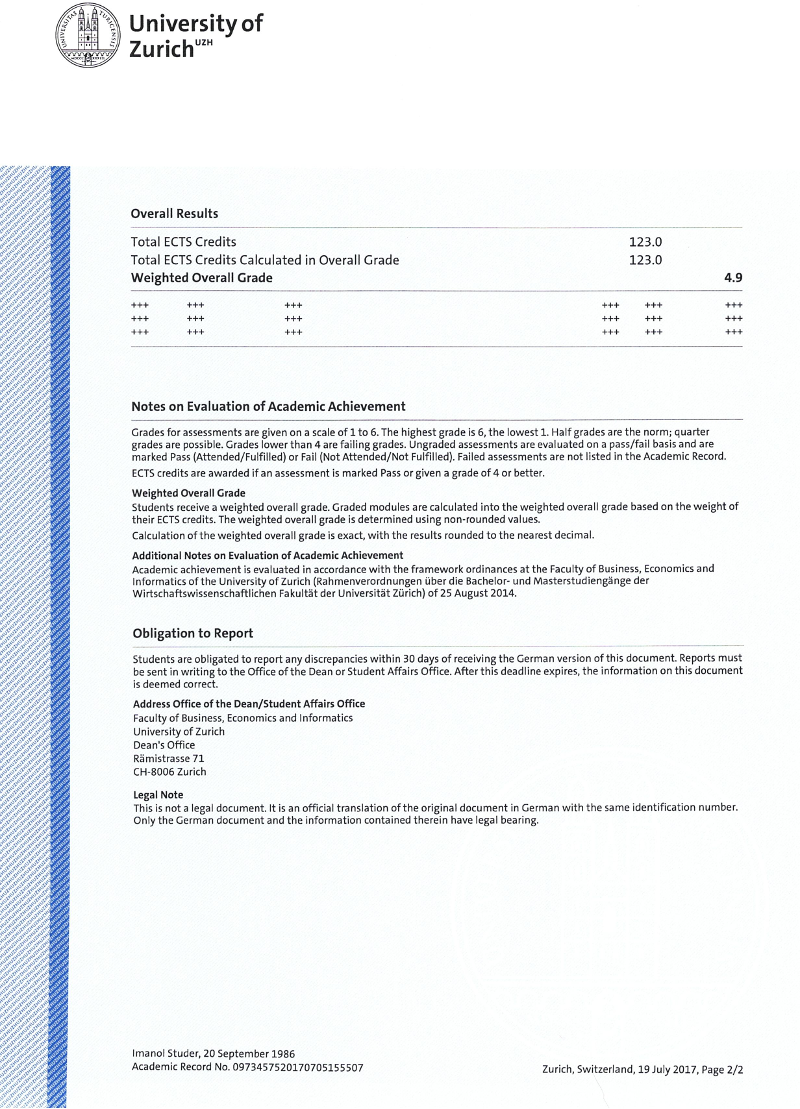
\includegraphics[width=\textwidth]{pictures/bachelor/page2.png}
\includegraphics[width=\textwidth]{pictures/bachelor/page3.png}

\restoregeometry

\end{document}